\paragraph{\trDehnTwist{}。}\label{sub:dehn-twists}
设 $M$ 是一个\trCorneredBoundary{}的\trExactSymplectic\trManifold{}。对任何带\trFrame{}的\trExact\trLagrange\trSphere{}$V\subset M$，都可以关联其\textbf{\trDehnTwist}（Dehn twist，亦称\trPicard--\trLefschetz{}变换）$\tau_V$，它是 $\operatorname{Aut}(M,\partial M)$ 的一个在相差\trIsotopy{}的意义下唯一的元素（更准确的说法是：构造 $\tau_V$ 时所作的那些额外选取的空间是\trContractible{}的）。为定义它，要用\trLagrange\trTubularNeighborhood{}定理，它把\trFrame{}$v\colon S\to V$ 扩张为一个\trSymplectic\trEmbedding{}$\psi\colon B_s^*S\to\mathrm{int}(M)$，其中 $B_s^*S$ 是 $S$ 上长度 $\le s$ 的那些\trCotangent{}向量构成的子集，$s>0$。现在取一个函数 $b\colon\RR\to\RR$ 满足
\begin{equation}\label{eq:dehn-twist-function}
\begin{cases}
b(r)=0 & \text{当 } r\ge s\text{ 时，以及} \\
b(r)-b(-r)=-r & \text{处处成立。}
\end{cases}
\end{equation}
在 $\psi(B_s^*S)\setminus V$ 上定义 $H(x)=b(|\psi^{-1}(x)|)$，并在 $M\setminus V$ 的其余部分上把它延拓为零。于是，$\tau_V$ 就是这个\trHamiltonian{}函数的时间 $2\pi$ \trFlow{}，它以唯一可能的方式延拓到 $V$ 本身之上。为了得到更具体的图像，回想 $T^*S\setminus S$ 上的长度函数 $|\xi|$ 的\trHamiltonian{}流可以等同于\trNormalization{}的\trGeodesic{}流（沿从该向量发出的\trGeodesic{}、以单位速度移动任何非零切向量，而不顾此向量的长度）。因此，$b(|\xi|)$ 的\trFlow{}以速度 $b'(|\xi|)$ 移动切向量。当长度趋于零时，导数趋于 $-1/2$，取极限便得到\trZeroSection{}上的\trAntipodal{}映射。为看出这个在\trZeroSection{}上的延拓是\trSmooth{}的（而不仅是连续的），写 $b(r)=\beta(r^2)-r/2$，其中 $\beta$ 是\trSmooth{}的（这是可能的，因为 $b(r)+r/2$ 是偶函数）。$\beta(|\xi|^2)$ 的\trFlow{}在整个\trCotangent{}丛上是\trSmooth{}的，而 $-|\xi|^2/2$ 的\trFlow{}则在时刻 $2\pi$ 变成\trAntipodal{}映射（此外，这两个\trHamiltonian{}量\trPoisson{}交换，因为二者都是 $|\xi|$ 的函数）。有鉴于此，可以把 $b(|\xi|)$ 的时间 $2\pi$ 映射写成两个\trSymplectic\trAutomorphism{}的\trComposition，其中每一个在\trZeroSection{}附近都显然是\trSmooth{}的。再稍微细看一下这个构造，就能发现 $\tau_V$ 实际上是\trExact{}的（这只在最低维数、即 $M$ 是一个\trSurface{}时才非平凡，所以也可以通过检视\trDehnTwist{}的标准图形来证明它）。按定义，$[\tau_V]\in\pi_0(\operatorname{Aut}(M,\partial M))$ 这个类在把 $V$ 当作带\trFrame{}的\trExact\trLagrange\trSphere{}所作的\trIsotopy{}下不变。特别地，它不依赖于 $V$ 的\trOrientation{}。
\begin{remark}\label{thm:dehn-twist-framing-independence}
$[\tau_V]$ 是否依赖于\trFrame{}，这个问题有些微妙。对\trFukayaCategory{}所诱导的\trAutoequivalence{}而言，已知\trFrame{}并不重要（在相差诸\trAFunctor{}的\trIsomorphism{}的意义下）。我们不打算证明这个命题，但它的一个弱版本（只涉及对\trObject{}的作用）可由推论 17.17 推出。
\end{remark}
取一个\trExact{}的\trLefschetzFibration{}$\pi\colon E\to S$ 与一条\trVanishingPath{}$\gamma$。设 $V_\gamma$ 是相伴的\trVanishingCycle{}，位于 $M=E_{\gamma(0)}$ 中。在 $S\setminus\mathrm{Critv}(\pi)$ 中取一条把 $\gamma$ 加倍的\trLoop{}$\lambda$，沿\trAnticlockwise{}方向绕 $\gamma(1)$ 盘绕（\cref{fig:dehn-twist-monodromy}）。那么绕 $\lambda$ 的\trMonodromy{}本质上就是沿 $V_\gamma$ 的一个\trDehnTwist{}，更确切地说，
\begin{equation}\label{eq:symplectic-picard-lefschetz}
h_\lambda\simeq\tau_{V_\gamma}
\end{equation}
其中 $\simeq$ 指 $\operatorname{Aut}(M)$ 中的\trIsotopy{}（如果按 \cref{thm:original-definition-remark} 的意义假设该\trFibration{}在 $\partial^hE$ 附近是平凡的，那么这个命题可以说得略微更精确些：该\trIsotopy{}将发生在群 $\operatorname{Aut}(M,\partial M)$ 之内）。这就是\textbf{\trSymplectic\trPicard--\trLefschetz{}定理}（symplectic Picard--Lefschetz theorem）。我们不在这里给出它的证明，但把基本策略概述一下或许值得。首先注意，对\trLefschetzFibration{}的结构作\trDeformation{}（在沿 $\partial^hE$ 表现良好的\trDeformation{}的意义下，见 \cref{sub:isomorphisms-deformations}）并不影响命题是否成立，因为它只通过一个\trIsotopy{}改变两侧。正如 \cref{sub:lefschetz-fibrations} 中提到的，可以找到这样一个\trDeformation，使得 $E$ 上的\trSymplecticStructure{}在该\trCriticalPoint{}周围的局部\trHolomorphic\trMorse{}\trChart{}中是标准的。在这样的局部坐标中，一条驶入该\trCriticalPoint{}的短路径的\trVanishingCycle{}可以显式写出，以\cref{thm:toy-model-thimble}为模型。类似地，沿该\trCriticalPoint{}周围一条充分小的\trCircle{}的\trMonodromy{}可以通过积分相应的\trVectorField{}来确定，结果就是沿该\trVanishingCycle{}的\trDehnTwist{}。然后，一个简单的\trParallelTransport{}论证便使人能够对原来的路径 $\gamma$ 与 $\lambda$ 推出相应的命题。
\begin{figure}[htbp]
\centering
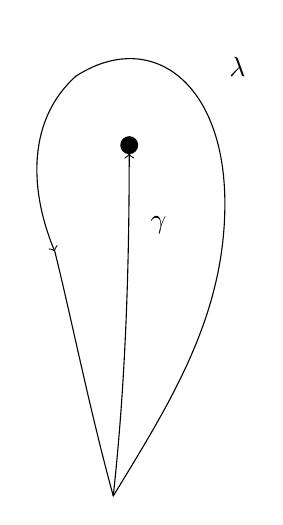
\begin{tikzpicture}[line cap=round,line join=round,scale=1.35]
\fill (0.15,3.3) circle (2.4pt);%
\draw[->,shorten >=3pt] (0,0) .. controls (0.12,1.1) and (0.15,2.2) .. (0.15,3.3);
\node[anchor=west] at (0.26,2.55) {$\gamma$};
\draw
  (0,0) .. controls (0.55,0.9) and (1.05,1.7) .. (1.05,2.75)
        .. controls (1.05,3.9) and (0.35,4.4) .. (-0.35,3.95);
\draw[->]
  (-0.35,3.95) .. controls (-0.8,3.55) and (-0.8,2.9) .. (-0.55,2.3);
\draw
  (-0.55,2.3) .. controls (-0.4,1.7) and (-0.22,0.8) .. (0,0);
\node[anchor=south west] at (1.0,3.85) {$\lambda$};
\end{tikzpicture}
\caption{}\label{fig:dehn-twist-monodromy}
\end{figure}
\begin{remark}\label{thm:picard-lefschetz-isotopy-uniqueness}
显然，用来证明 \eqref{eq:symplectic-picard-lefschetz} 的那个\trDeformation{}并非完全唯一，但可能选取的空间是\trContractible{}的。这表明，在这两个\trSymplectic\trAutomorphism{}之间，（相对端点）的\trIsotopy{}的\trHomotopy{}类实际上是唯一的。
\end{remark}
